\documentclass[12pt, letterpaper]{article}
%\documentclass[12pt, letterpaper]{amsart}

%%%%%%%%%%%% LANGUAGE & ENCODING %%%%%%%%%%%%%%%%%
\usepackage[english]{babel}
\usepackage[utf8]{inputenc}%%%% to process umlauts and accents directly
%\usepackage{indentfirst}
%\usepackage{ucs}

%%%%%%%%%%% PACKAGES %%%%%%%%%%%%%%%%%%%%%%%%%%%%%
% For Hyperlinks
\usepackage[colorlinks,linkcolor=cyan,citecolor=magenta]{hyperref}

% Common math packages
\usepackage{amsthm, amsmath, amsfonts, amssymb, esint, mathrsfs, mathtools}
\usepackage{tensor} % To handle multi-index notation
\usepackage[capitalize,nameinlink]{cleveref} % Nice references
\crefname{equation}{}{} % Removes Eq. from equation references
\numberwithin{equation}{section} % Number equations within each section separately

% Extra symbols
\usepackage{stmaryrd} % contains \owedge  for Kulkarni-Nomizu product and some other special characters
\usepackage{commath} % contains \norm \abs

% Some useful packages
\usepackage{verbatim} %%% enables \begin{comment}    \end{comment}
\usepackage{enumerate} % allows different types of indices
\usepackage{float} % Handling figures

%%%%%%%%%%% MARGINS %%%%%%%%%%%%%%%%%%%%%%%%%%%%%%%%
% Margins
\usepackage[top=1in, bottom=1in, left=1in, right=1in]{geometry}

%%%%%%%%%%% CUSTOM NOTATION  %%%%%%%%%%%%%%%%%%%%%%
\newcommand{\N}{\mathbb{N}}
\newcommand{\Z}{\mathbb{Z}}
\newcommand{\Q}{\mathbb{Q}}
\newcommand{\R}{\mathbb{R}}
\newcommand{\C}{\mathbb{C}}
\newcommand{\K}{\mathbb{K}}

\newcommand{\f}{\mathfrak}
\newcommand{\ul}{\underline}
\newcommand{\mb}{\mathbb}
\newcommand{\mr}{\mathrm}
\newcommand{\mf}{\mathbf}
\newcommand{\mc}{\mathcal}
\newcommand{\e}{\emph}
\newcommand{\vp}{\varphi}
\newcommand{\ve}{\varepsilon}

\newcommand{\vol}{\operatorname{Vol}}
\newcommand{\diam}{\operatorname{diam}}
\newcommand{\dist}{\operatorname{dist}}
\newcommand{\dv}{\operatorname{div}}
\newcommand{\tr}{\operatorname{tr}}

\newcommand{\dd}{\; \mathrm{d}} %%%% d for integration dx
\newcommand{\wt}{\widetilde}
\newcommand{\ol}{\overline}

%%%%%%%%%%% THEOREMS %%%%%%%%%%%%%%%%%%%%%%%%
\newtheorem{theorem}{Theorem}[section]
\newtheorem{lemma}[theorem]{Lemma}
\newtheorem{proposition}[theorem]{Proposition}
\newtheorem{conjecture}[theorem]{Conjecture}
\newtheorem{corollary}[theorem]{Corollary}
\newtheorem{claim}[theorem]{Claim}
\newtheorem{problem}[theorem]{Problem}
\newtheorem{remark}[theorem]{Remark}

\theoremstyle{definition}
\newtheorem{definition}[theorem]{Definition}

\theoremstyle{remark}
\newtheorem{example}[theorem]{Example}


%%%%%%%%%%% TITLE %%%%%%%%%%%%%%%%%%%
%\title[CIS625: Computational Learning Theory]{Computational Learning Theory Lecture Notes}
%\author[Notes by Martin Citoler-Saumell]{Martin Citoler-Saumell}
%\date{Spring 2017}
%\address{University of Pennsylvania\\ Philadelphia, PA 19104}
%\email{\href{mailto:martinci@math.upenn.edu}{martinci@math.upenn.edu}}

\title{Computational Learning Theory Lecture Notes}
\author{Martin Citoler-Saumell}
\date{CIS625 Spring 2017}

%%%%%%%%%%% DOCUMENT BEGINS %%%%%%%%%%%%
\begin{document}
%------------------------------------------------------------
%          LECTURE 6
%------------------------------------------------------------
\section{Lecture 6: 2017.02.27}

\subsection{Learning with Noise}
Now we turn our attention to learning with noise. The set up is the same as in the PAC-learning with the difference that the ``subroutine'' that extracts examples, $EX_\eta(c,D)$, is now a Bernoulli trial. With probability $1-\eta$ it returns the correct label $\langle x, c(x) \rangle$ and with probability $\eta$ it returns the incorrect label $\langle x, \lnot c(x) \rangle$. We also ask for the algorithm to be polynomial on $\frac1{1-2\eta}$.
\begin{itemize}
\item We assume that the noise is \emph{independent} of $x$ and $c(x)$. This is akin to measurement error. Note that our noise affects only the labels and not on the $x$'s.
\item We also assume that $\eta < \frac12$. Otherwise it would be impossible to distinguish between the true label and the false label.
\end{itemize}
\begin{figure}[H]
\centering
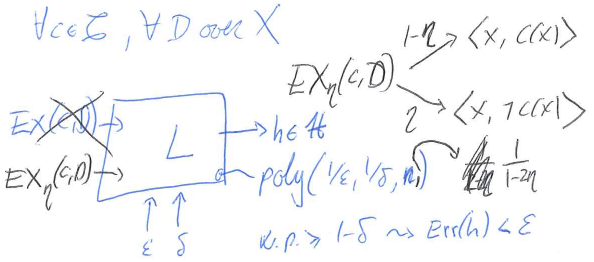
\includegraphics[width=0.6\linewidth]{img/noise-pac.png}
\caption{PAC-learning with noise.}
\end{figure}

Given any $h\in \mc H$, we can compute the noisy error
\begin{align}
\mb P_{\langle x, y\rangle \sim EX_\eta}[h(x)\ne y] = (1-\eta)Err(h) + \eta(1-Err(h)) = \eta + (1-2\eta)Err(h),
\end{align}
observe that since we have $\eta < \frac12$, this is increasing as a function $Err(h)$. This means that noise preserves the ranking of hypothesis according to their error. So we can still minimize this quantity and obtain a good model.
\begin{remark}
As a consequence, all the VCD results still hold with the only caveat that we need more data, in particular, we need 
\begin{align}
m \sim \frac{VCD(\mc C)}{\ve^2(1-2\eta)^2}\log\left(\frac1\delta\right).
\end{align}
\end{remark}

\subsubsection{``Malicious'' Errors}
Same setup as before but with a slight change.
\begin{itemize}
\item with probability $1-\eta$ we return the correct pair $\langle x, c(x)\rangle$,
\item with probability $\eta$, an ``adversary'' generates \emph{any} pair $\langle x, y\rangle$.
\end{itemize}
The general theory still applies and by minimizing observed error we can still pick up a target with error at most $\eta$. However, the ``malicious'' problem is considerably worse and we can no longer ask for $Err << \eta$. To see this consider a fixed distribution $D$ over X and two concepts $c_1, c_2 \in \mc C$ such that $c_1 \triangle c_2$ has $\ve$ weight under $D$. \\
\begin{figure}[H]
\centering
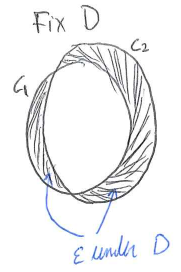
\includegraphics[width=0.3\linewidth]{img/malicious.png}
\caption{Malicious noise.}
\end{figure}
Then, as long as $\eta \geq \frac \ve{1+\ve}$, the adversary can make you confuse $c_1$ and $c_2$. 

\subsection{Learning (monotone) Conjunctions with ``Statistics''}
Recall the problem of learning conjunctions.
\begin{itemize}
\item $X=\lbrace 0, 1\rbrace^n$, concept class. E.g. $c=x_1\land x_5\land x_6\land x_{19}$.
\end{itemize}
We started with the hypothesis $h=x_1\land\ldots\land x_n$ and we deleted any variable that contradicted the positive examples (all the variables that are zero in some positive example). However, if we introduce noise this algorithm falls apart since we could have the all 0's vector to be incorrectly labeled positive which results in the empty conjunction. The underlying problem is that we made drastic decisions on our hypothesis based on a single examples. To overcome this shortcoming, we will only introduce changes if we see enough \emph{statistical} evidence.
\begin{itemize}
\item For each $x_i$, define
\begin{align}
p_0(x_i) &= \mb P_{\vec x\sim D}[x_i=0],\\
p_{01}(x_i) &= \mb P_{\vec x\sim D}[x_i=0 \;\&\; c(\vec x) = 1].
\end{align}
We call $x_i$ \emph{significant} if $p_0(x_i) \geq \frac\ve{4n}$, and \emph{harmful} if $p_{01}(x_i) \geq \frac\ve{4n}$.

\item \ul{Algorithm:} Let $h$ be the conjunction of all $x_i$'s that are significant and not harmful.
\end{itemize}
Let's look at the analysis of the errors. For the FP type
\begin{align}
\mb P_{\vec x \sim D}[c(\vec x)=0 \;\&\; h(\vec x)=1],
\end{align}
must be some $x_i$ such that $x_i \in c$, $c_i\not \in h$ and $x_i=0$. This means that $x_i$ is not harmful which implies that $x_i$ is not significant and $p_0(x_i)\leq \frac\ve{4n}$. Thus, the total error  is $p_0(n)\leq n \frac\ve{4n} \leq \frac\ve4$. Similarly, for the FN type
\begin{align}
\mb P_{\vec x \sim D}[c(\vec x)=1 \;\&\; h(\vec x)=0],
\end{align}
must be some $x_i$ such that $x_i\not\in c$, $x_i\in h$ and $x_i=0$. Therefore, $p_{01}(n) \leq \frac\ve{4n} n \leq \frac\ve4$.
\begin{remark}
\begin{remark}[Concentration Inequalities]
Consider a biased coin with $\mb P[head] = p$ and $\mb P[tails]=1-p$. We flip the coin $m$ times and let $\hat p = \frac{\textrm{\# heads observed}}{m}$. We are interested in bounds like (Hoeffding's)
\begin{align}
\mb P_{\textrm{m flips}}\left[\abs{p-\hat p}\geq \ve\right] \leq e^{-\frac{\ve^2m}{3}},
\end{align}
and the closely related Chernoff bound. This is like the law of large numbers but with an explicit rate.
\end{remark}
We can estimate the $p_0(x_i)$ probabilities with $EX_\eta(c, D)$ since we don't care about the noise of the labels.
\end{remark}
The interesting part is that we can do the same for the $p_{01}$'s.

\subsection{Statistical Query (SQ) Learning}
\begin{remark}[Warning]
The professor sort of rushed through the definition of SQ-learning. Check the textbook for more details.
\end{remark}
We modify the PAC learning algorithm. We replace the subroutine $EX(c,D)$ with $SQ(c,D)$ which interacts with the algorithm $L$ in the role of ``oracle'', answering the questions (queries) posed by $L$. For example, what is the probability of $x_i=0$?.

These queries, $\chi$, are \emph{predicates} ($0/1$ valued functions) on $\langle x, y\rangle$ pairs
\begin{align}
\chi(x,y)\in \lbrace 0, 1\rbrace^n \longrightarrow P_{\chi} \coloneqq \mb P_{\langle x,y\rangle\sim EX(c,D)}[\chi(x,y)=1].
\end{align}
E.g. $\chi(\vec x, y) = 1 \iff x_{11}=0$ [$p_{0}(x_{11})$]\\
E.g. $\chi(\vec x, y) = 1 \iff x_{11}=0$ \& $y=1$ [$p_{01}(x_{11})$]

On query $\chi$, $SQ(c,D)$ returns any value $\hat P_\chi  \in \left[P_\chi -\tau, P_\chi +\tau\right]$. To say that $\mc C$ is \emph{SQ-learnable} if  we require $\tau \geq poly\left(\frac\ve n\right)$
\begin{figure}[H]
\centering
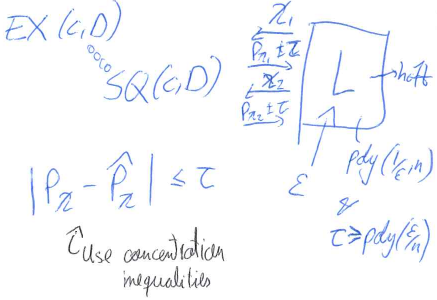
\includegraphics[width=0.6\linewidth]{img/sq-learning.png}
\caption{Statistical Query Learning.}
\label{fig:graph}
\end{figure}


\begin{theorem}[uninteresting]
    If $\mc C$ is SQ-learnable, then $\mc C$ is PAC-learnable.
\end{theorem}

\begin{theorem}
    If $\mc C$ is SQ-learnable, then $\mc C$ is PAC-learnable \ul{with} noise.
\end{theorem}
\begin{proof}
    We want to estimate
    \begin{align}
    P_\chi \coloneqq \mb P_{\langle x,y\rangle\sim EX(c,D)}[\chi(x,c(x))=1],\\
    P_\chi^\eta \coloneqq \mb P_{\langle x,y\rangle\sim EX^\eta(c,D)}[\chi(x,y)=1],
    \end{align}
    but we don't have access to the $EX(c,D)$ subroutine. Consider
    \begin{align}
    X_2 \coloneqq \lbrace x\in X \;:\; \chi(x,0)= \chi(x,1)\rbrace,
    \end{align}
    and define the following partition of $X$
    \begin{align}
    X_1 \coloneqq \lbrace x\in X \;:\; \chi(x,0)\ne \chi(x,1)\rbrace,
    \end{align}
    $X_1$ and $X_2$ are disjoint and clearly  $X_1\cup X_2 = X$. Now consider $p_1 = D[X_1]$ and $p_2 = 1 - p_1 =  D[X_2]$. For $x\in X$ we have the normalized conditioned distributions
    \begin{align}
    D_1[X] = \frac{D[X]}{p_1}\rightarrow P_\chi^1 = \mb P_{EX(c,D_1)}[\chi=1],\\
    D_2[X] = \frac{D[X]}{p_2}\rightarrow P_\chi^2 = \mb P_{EX(c,D_2)}[\chi=1].
    \end{align}
    This just introduced notation. By considering conditioned probabilities, we now can compute
    \begin{align}
    P_\chi^\eta &= (1-\eta)P_\chi + \eta\left(p_1\underbrace{\mb P_{x\sim D_1,y=\lnot c(x)}[\chi(x,y)=1]}_{\mb P_{EX(c,D)}[\chi(x, c(x))=0] \eqqcolon 1 - P_\chi^1} + p_2\underbrace{\mb P_{x\sim D_2,y=\lnot c(x)}[\chi(x,y)=1]}_{\mb P_{EX(c,D_2)}[\chi(x,c(x))=1] \eqqcolon P_\chi^2}\right)\\
    &=(1-\eta)P_\chi + \eta\left(p_1(1 - P_\chi^1) + p_2 P_\chi^2\right).
    \end{align}
    We can solve this for $P_\chi$
    \begin{align}
    P_\chi = \frac1{1-\eta}\left[P_\chi^\eta -\eta\left(p_1(1 - P_\chi^1) + p_2 P_\chi^2\right)\right].
    \end{align}
    Bu now we can empirically estimate all the elements in the RHS using noisy data. The only tricky one is $P_\chi^1$ but we have
    \begin{align}
    P_\chi^1 = \frac{P_\chi^\eta - p_2P_\chi^2 -\eta p_1}{(1-2\eta)p_1},
    \end{align}
    so we are fine. To finish the proof in detail one has to do a robustness analysis of the expression that we are using to estimate $P_\chi$. See the textbook for more details.
\end{proof}

\begin{claim}
``Almost'' every PAC-learning algorithm has an SQ-algorithm.
\end{claim}

We can actually find counterexamples to the claim, hence the ``almost'' in the statement.
\subsubsection{PAC-learnable but not SQ-learnable}
Consider the space $X=\lbrace 0,1 \rbrace$. For any subset $S\subset \lbrace 1,\ldots, n\rbrace$ we can define the functions
\begin{align}
f_S(\vec x) = \sum_ic_ix_i \mod 2 = \bigoplus\limits_{i\in S} x_i,
\end{align}
and the associated pairs $\langle \vec x, f_S(\vec x)\rangle$. In turns out that this is PAC-learnable because examples correspond to linear equations but you can't can get the same information statistically.
\end{document}
